A continuación presentaremos las técnicas mencionadas con su respectivo análisis:

\subsection{Vecinos}
El primer método que analizaremos será el de vecinos. Este consiste en rellenar los valores de cada una de las columnas
nuevas de la imagen replicando su valor más próximo. La principal ventaja de este metodo es la simpleza de su implementación, que consta unicamente de dos bucles para iterar la matriz original. Caracteristica que ademas le provee de una eficiencia del orden de O($n^2$) siendo n el alto y ancho de la imagen destino.

\begin{algorithm}
\begin{algorithmic}[1]\parskip=1mm
\caption{void vecinos(Matriz *image, Matriz *imageRes , int k)}
\FOR{0 \TO imageRes$\rightarrow$rows}
    \FOR{0 \TO imageRes$\rightarrow$cols}
        \STATE{imageRes$\rightarrow$at(i, j) $=$ image$\rightarrow$at(round(i/(k+1)), round(j/(k+1)))\\}
    \ENDFOR
\ENDFOR
\end{algorithmic}
\end{algorithm}

Como se menciono anteriormente, a pesar su alta eficiencia temporal comparado con los demas metodos, nuestra intuicion nos dice que este va ser el que presente una mayor cantidad de ruido, debido a que simplemente se estan replicando los pixeles de las imgenes. Como resultado, teniendo en cuenta que lo unico que se logra es 'anadir grosor' a los pixeles, deberian conseguirse imagenes de mayor tamaño pero con una ganancia igual de rapida en los valores de ruido a medida que los valores de $k$ aumentan.

\subsection{Interpolación bilineal}
El segundo método que analizaremos será el de interpolación bilineal. En este caso, la idea consiste en generar un polinomio entre
dos puntos consecutivos de la imagen para, por medio de este, calcular los valores necesarios para la extensión. \\
Primero realizaremos el cálculo por filas y una vez calculados estos valores, repetiremos el mismo procedimiento por columnas.
Sean entonces $Q_{11}$, $Q_{12}$, $Q_{21}$, $Q_{22}$ los cuatro puntos de la imagen original sobre los que queremos interpolar, el objetivo es conseguir un polinomio P que valga lo mismo en cada uno de estos puntos y aproxime los nuevos valores intermedios. Usaremos entonces para esto el polinomio interpolador de Lagrange.

Interpolando entonces en el eje X obtenemos la siguiente formula:

\begin{center}
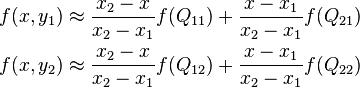
\includegraphics[scale=0.75]{imagenes/bilinealX.png}\\
\end{center}


Ahora, realizando el mismo procedimiento pero en el eje Y, obtenemos lo siguiente:

\begin{center}
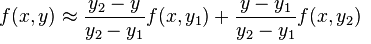
\includegraphics[scale=0.75]{imagenes/bilinealY.png}\\
\end{center}

Si notamos, los puntos que acompañan a las bases polinómicas de Lagrange son los mismos que calculamos sobre el eje X, por lo que podemos realizar el remplazo para llegar a una formula cerrada:

\begin{center}
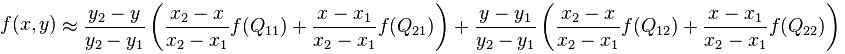
\includegraphics[scale=0.75]{imagenes/bilinealXY.png}\\
\end{center}

Distribuyendo los valores dentro de los paréntesis, obtenemos la ecuación final

\begin{center}
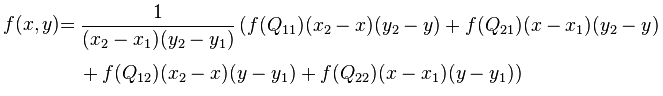
\includegraphics[scale=0.75]{imagenes/bilinealFinal.png}\\
\end{center}

Notese que se obtiene el mismo polinomio interpolador tanto si se hace primero sobre el eje X y luego sobre el Y, como a la inversa. Ahora, gracias a este polinomio interpolador, podemos conseguir los valores de las posiciones $(x,y)$ que agregamos a nuestra imagen para realizar el zoom.
Para facilitar la lectura y escritura del ejercicio vamos a definir una estructura que se llama punto que dentro de la misma vamos a tener los 3 valores, el primero es el valor en x, el segundo en y y el tercero un valor que sera de la imagen original. 
En el siguiente codigo las variables q11,q12,q21,q22 son del tipo descripto anteriormente y se utilizan para definir los 4 puntos en los cuales se va a realizar el polinomio interpolador.
%TODO PSEUDOCODIGO
\begin{algorithm}
\begin{algorithmic}[1]\parskip=1mm
\caption{void bilineal(matriz A, vector Res,int k)}
  \STATE{Para i$=0...CantFilas$}
  \STATE{\quad Para j$=0...CantColumnas$}
  \STATE{\quad \quad q11 = $<0,0, A_{i,j}>$}
  \STATE{\quad \quad q12 = $<0,k+1, A_{i,j+1}>$}
  \STATE{\quad \quad q21 = $<k+1,0, A_{i+1,j}>$}
  \STATE{\quad \quad q22 = $<k+1,k+1, A_{i+1,j+1}>$}
  \STATE{\quad \quad Para x=$0...k+1$}
  \STATE{\quad \quad \quad Para y=$0...k+1$}
  \STATE{\quad \quad \quad \quad valorRes $=$ poliniomioInterpolador(q11,q12,q21,q22,x,y) }
  \STATE{\quad \quad \quad \quad $Res_{i*(k+1)+x,j*(k+1)+y} =$ valorRes}
\end{algorithmic}
\end{algorithm}\\
Donde polinomio interpolador es la funcion que se encarga de generar el polinomio interpolador en el punto, De la siguiente manera.
\begin{algorithm}
\begin{algorithmic}[1]\parskip=1mm
\caption{void polinomioInterpolador(punto q11,punto q12, punto q21, punto q22, int x, int y)}
  \STATE{denominador = 1/ ((q22.x-q11.x)* (q22.y-q11.y)) }
  \STATE{numerador1= q11.valor* (q22.x-res.x)*(q22.y-res.y) + q21.val * (res.x-q11.x)*(q22.y-res.y)}
  \STATE{numerador2= q12.valor* (q22.x-res.x)*(res.y-q11.y) + q22.val * (res.x-q11.x)*(res.y-q11.y)}
  \STATE{retorno ((numerador1+numerador2)*denominador)}
\end{algorithmic}
\end{algorithm}

\subsection{Interpolación por Splines}
Por último nos centraremos en la interpolación por Splines. Este método, similar al anterior, requiere el cálculo de Splines (al igual que antes, por filas y luego por columnas) para obtener los valores de los casilleros a extender.
Además, en este caso, dado que la interpolación por medio de Splines trata de generar polinomios para un segmento
específico de la imagen, también analizaremos una versión en la cual el Spline calculado solo incluye los valores de un recuadro de tamaño menor, dejando de lado los valores de la imagen externos (que están influyendo sobre un polinomio que intenta interpolar valores posiblemente lejos de los suyos).

Sea $S_{j}(x) = a_{j} + b_{j}(x - x_{j}) + c_{j}(x - x_{j})^2 + d_{j}(x - x_{j})^3$ nuestro polinomio interpolador para cada $j$ intervalo entre $0$ y $n-1$, necesitamos entonces resolver los coeficientes. Utilizamos la construcción de Splines despejando estos ultimos en funcion de $c_{j}$ para formar el siguiente sistema de ecuaciones $Ax = b$:

\begin{center}
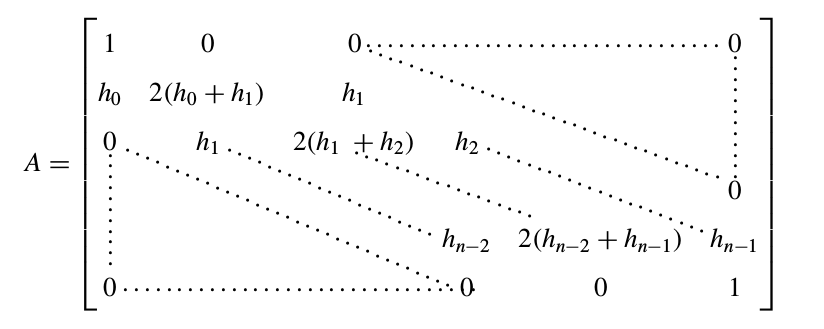
\includegraphics[scale=0.50]{imagenes/A.png}
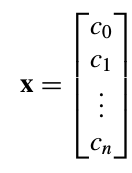
\includegraphics[scale=0.50]{imagenes/x.png}
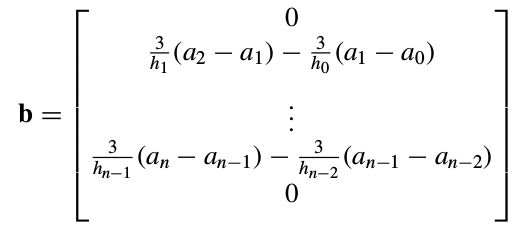
\includegraphics[scale=0.50]{imagenes/b.png}
\end{center}

donde $h = x_{j+1} - x_{j}$. Para nuestra aplicacion $h = k$ y se mantiene fijo, ya que la distancia entre los puntos de la nueva imagen es igual a $k$. Una vez resuelto este sistema y con los valores de $c_{0},..., c_{n}$ ya calculados, podemos despejar los coeficientes que necesitabamos en base a las siguientes ecuaciones (que se derivan de las condiciones del mismo spline):

$a_j$ es el valor del pixel en la posicion $j$ de la imagen original en la fila o columna iterada por el spline \\
$b_{j} = \frac{1}{k}(a_{j+1} - a_j) - \frac{k}{3}(2c_j + c_{j+1})$ \\
$d_{j} = \frac{c_{j+1} - c_{j}}{3k} $ \\

%TODO PSEUDOCODIGO

\subsection{Interpolación por Splines}
Por último nos centraremos en la interpolación por Splines. Este método, similar al anterior, requiere el cálculo de Splines (al igual que antes, por filas y luego por columnas) para obtener los valores de los casilleros a extender.
Además, en este caso, dado que la interpolación por medio de Splines trata de generar polinomios para un segmento
específico de la imagen, también analizaremos una versión en la cual el Spline calculado solo incluye los valores de un recuadro de tamaño menor, dejando de lado los valores de la imagen externos (que están influyendo sobre un polinomio que intenta interpolar valores posiblemente lejos de los suyos).

Sea $S_{j}(x) = a_{j} + b_{j}(x - x_{j}) + c_{j}(x - x_{j})^2 + d_{j}(x - x_{j})^3$ nuestro polinomio interpolador para cada $j$ intervalo entre $0$ y $n-1$, necesitamos entonces resolver los coeficientes. Utilizamos la construcción de Splines despejando estos ultimos en funcion de $c_{j}$ para formar el siguiente sistema de ecuaciones $Ax = b$:

\begin{center}
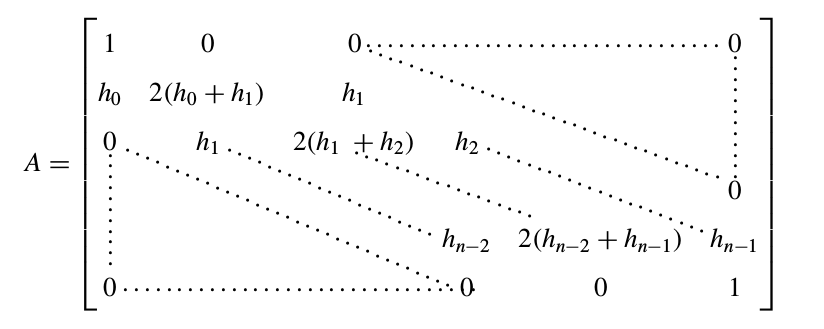
\includegraphics[scale=0.50]{imagenes/A.png}
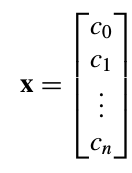
\includegraphics[scale=0.50]{imagenes/x.png}
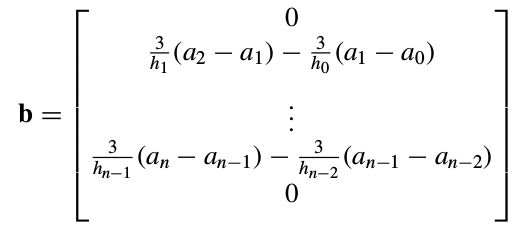
\includegraphics[scale=0.50]{imagenes/b.png}
\end{center}

donde $h = x_{j+1} - x_{j}$. Para nuestra aplicacion $h = k$ y se mantiene fijo, ya que la distancia entre los puntos de la nueva imagen es igual a $k$. Una vez resuelto este sistema y con los valores de $c_{0},..., c_{n}$ ya calculados, podemos despejar los coeficientes que necesitabamos en base a las siguientes ecuaciones (que se derivan de las condiciones del mismo spline):

$a_j$ es el valor del pixel en la posicion $j$ de la imagen original en la fila o columna iterada por el spline \\
$b_{j} = \frac{1}{k}(a_{j+1} - a_j) - \frac{k}{3}(2c_j + c_{j+1})$ \\
$d_{j} = \frac{c_{j+1} - c_{j}}{3k} $ \\

%TODO PSEUDOCODIGO


En este metodo, comparado con el anterior que solo replicaba pixeles vecinos, se esta calculando un polinomio para tratar de introducir cierto nivel de suavidad entre los de la imagen original a medida que se atraviezan los pixeles agregamos. Un dato importante a tener en cuenta es que dado que el grado del polinomio aumenta a medida que la cantidad de puntos a interpolar lo hace, decidimos que esta se realice entre solo dos puntos de la imagen original, para ofrecer un mejor desempe\~no entre puntos, haciendo que el polinomio calculado sea mas operativo y evitando que este osile demasiado (situacion conocida como Fenomeno de Runge\footnote{\url{https://es.wikipedia.org/wiki/Fenomeno_de_Runge}}). Como contrapartida de esta optimizacion, es necesario recalcular el polinomio interpolador para todo par de puntos entre la imagen pero teniendo en cuenta que no se trabaja con imagenes de una definicion desmesurada, es un costo que se puede pagar en detrimento de los beneficios obtenidos.

\subsection{Interpolación por Splines}
Por último nos centraremos en la interpolación por Splines. Este método, similar al anterior, requiere el cálculo de Splines (al igual que antes, por filas y luego por columnas) para obtener los valores de los casilleros a extender.
Además, en este caso, dado que la interpolación por medio de Splines trata de generar polinomios para un segmento
específico de la imagen, también analizaremos una versión en la cual el Spline calculado solo incluye los valores de un recuadro de tamaño menor, dejando de lado los valores de la imagen externos (que están influyendo sobre un polinomio que intenta interpolar valores posiblemente lejos de los suyos).

Sea $S_{j}(x) = a_{j} + b_{j}(x - x_{j}) + c_{j}(x - x_{j})^2 + d_{j}(x - x_{j})^3$ nuestro polinomio interpolador para cada $j$ intervalo entre $0$ y $n-1$, necesitamos entonces resolver los coeficientes. Utilizamos la construcción de Splines despejando estos ultimos en funcion de $c_{j}$ para formar el siguiente sistema de ecuaciones $Ax = b$:

\begin{center}
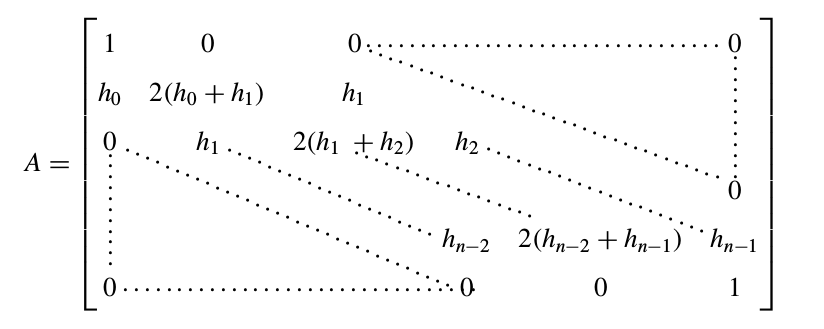
\includegraphics[scale=0.50]{imagenes/A.png}
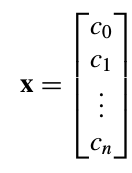
\includegraphics[scale=0.50]{imagenes/x.png}
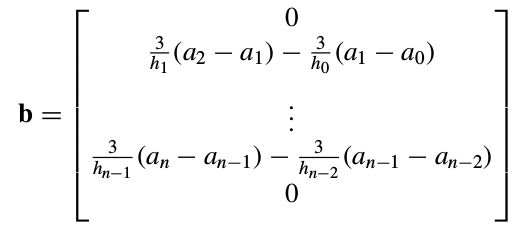
\includegraphics[scale=0.50]{imagenes/b.png}
\end{center}

donde $h = x_{j+1} - x_{j}$. Para nuestra aplicacion $h = k$ y se mantiene fijo, ya que la distancia entre los puntos de la nueva imagen es igual a $k$. Una vez resuelto este sistema y con los valores de $c_{0},..., c_{n}$ ya calculados, podemos despejar los coeficientes que necesitabamos en base a las siguientes ecuaciones (que se derivan de las condiciones del mismo spline):

$a_j$ es el valor del pixel en la posicion $j$ de la imagen original en la fila o columna iterada por el spline \\
$b_{j} = \frac{1}{k}(a_{j+1} - a_j) - \frac{k}{3}(2c_j + c_{j+1})$ \\
$d_{j} = \frac{c_{j+1} - c_{j}}{3k} $ \\

%TODO PSEUDOCODIGO


Este metodo, que podria considerarse un refinamiento del anterior, introduce la particularidad de que se le pide al polinomio interpolador que las intersecciones de las funciones que interpolan al punto $n-1$ y $n$ y al $n$ y al $n+1$, sean derivables. Como resultado, se agrega mucha mas suavidad entre puntos que con la tecnica anterior que solo respetaba que las funciones empiecen y terminen en el mismo punto (dando lugar a posibles picos, como en el caso de que dos puntos se interpolen con una recta ascendente y los siguientes con una descendente). Ademas, esta tecnica evita de forma natural la oscilacion del polinomio mencionada en el metodo anterior dado que siempre se toman polinomios por partes. Gracias a esto, cuando se intenta reducir el error de interpolación se puede incrementar el número de partes del polinomio que se usa para construir el spline, en lugar de incrementar su grado.
